%-----------------------------------------------------------------%
% 2015 - 2023 Emerson Ribeiro de Mello - mello@ifsc.edu.br
% 
% 2023/04/10 versão 1.01
% 
% Modelo de monografia para o Instituto Federal de Santa Catarina
% 
% Adaptação do documento abnTeX2: Modelo de Trabalho Acadêmico
% para ficar de acordo com o "Template para elaboração de trabalho 
% acadêmico" fornecido pela Biblioteca do IFSC 
% https://www.ifsc.edu.br/documentos-uteis. Acesso em 2022-08-27
% 
%-----------------------------------------------------------------%
\documentclass[
	12pt,				% tamanho da fonte
	openright,			% capítulos começam em pág ímpar (insere página vazia caso preciso)
	oneside,			% para impressão em recto e verso. Oposto a oneside
	a4paper,			% tamanho do papel. 
	% -- opções da classe abntex2 --
	chapter=TITLE,		% títulos de capítulos convertidos em letras maiúsculas
	%english,			% idioma adicional para hifenização
	% french,				% idioma adicional para hifenização
	% spanish,			% idioma adicional para hifenização
	brazil				% o último idioma é o principal do documento
	]{ifscthesis}


%-----------------------------------------------%
% Capa
%-----------------------------------------------%

%-----------------------------------------------%
% Para alterar o gênero dos comandos orientador
% e coorientador.
%-----------------------------------------------%
% \renewcommand{\orientadorname}{Orientadora:}
%\renewcommand{\coorientadorname}{Coorientadora:}
%-----------------------------------------------%


%-----------------------------------------------%
% Informações de dados para CAPA e FOLHA DE ROSTO
%-----------------------------------------------%
\titulo{Transferência de Calor com Superfícies Estendidas}
\autor{Ana Caroline Vidotti Ferreira\\
Gabriel Cabral Ferreira\\
Lucas Alves de Lima\\
Lucas de Jesus Wrubleski
}
\local{Jaraguá do Sul - SC}
\data{junho/2023}
\instituicao{
  Instituto Federal de Santa Catarin -- IFSC
  \par
  Campus Jaraguá do Sul - Rau
  \par
  Engenharia Elétrica}
\tipotrabalho{trabalho}
%-----------------------------------------------%




%-----------------------------------------------%
% O preambulo deve conter o tipo do trabalho, o objetivo, o nome da instituição e a área de concentração 
\preambulo{Trabalho apresentado pelos discentes do Curso de Engenharia Elétrica, 5ª Fase, como quesito avaliativo à disciplina de Fenômenos de Transporte do Instituto Federal de Santa Catarina - Campus Jaraguá do Sul - Rau e supervisionado pelo Professor Anderson José Antonietti.}

%\textoaprovacao{Este trabalho foi julgado adequado para obtenção do título de Engenheiro de Telecomunicações, pelo Instituto Federal de Educação, Ciência e Tecnologia de Santa Catarina, e aprovado na sua forma final pela comissão avaliadora abaixo indicada.}
%-----------------------------------------------%

%-----------------------------------------------%
% Estilo de cabeçalho que só contém o número da 
% página e uma linha
%-----------------------------------------------%
\makepagestyle{cabecalholimpo}
\makeevenhead{cabecalholimpo}{\thepage}{}{} % páginas pares
\makeoddhead{cabecalholimpo}{}{}{\thepage} % páginas ímpares
% \makeheadrule{cabecalholimpo}{\textwidth}{\normalrulethickness} % linha
%-----------------------------------------------%


%-----------------------------------------------%

%-----------------------------------------------%
% Incluir arquivo com acrônimos e símbolos
%-----------------------------------------------%
% 
% ATENÇÃO. Este projeto faz uso do pacote glossaries.
% Se for usar uma instalação local do LaTeX para
% compilar, e não no Overleaf, então é necessário 
% que tenha o arquivo .latexmkrc dentro diretório 
% deste projeto e use o comando abaixo:
% 
% latexmk -outdir=out -pdf monografia.tex
% 
% A extensão LaTeX Workshop do Visual Studio Code
% usa por padrão o latexmk para compilar
\makeglossaries


\newacronym
{json} % rótulo 
{JSON} % sigla
{\textit{JavaScript Object Notation}} % por extenso

\newacronym{ABNT}{ABNT}{Associação Brasileira de Normas Técnicas}

\newacronym{abnTeX}{abnTeX}{ABsurdas Normas para TeX}

\newacronym[longplural={Autoridades Certificadoras}]{AC}{AC}{Autoridade Certificadora}

\newacronym{AES}{AES}{\textit{Advanced Encryption Standard}}

\newacronym{TLS}{TLS}{\textit{Transport Layer Security}}

\newacronym{TPC}{TPC}{Terceira Parte Confiável}

\newacronym{IFSC}{IFSC}{Instituto Federal de Santa Catarina}
\glsxtrnewsymbol[description={conjunto vazio}]
{emptyset}% rótulo (será usado na ordenação na lista de símbolos)
{\ensuremath{\emptyset}}% símbolo


\glsxtrnewsymbol[description={número Pi}]
{pi}% rótulo (será usado na ordenação na lista de símbolos)
{\ensuremath{\pi}}% símbolo



%-----------------------------------------------%
% Início do documento
%-----------------------------------------------%
\begin{document}
% Seleciona o idioma do documento (conforme pacotes do babel)
\selectlanguage{brazil}




%-----------------------------------------------%
% ELEMENTOS PRÉ-TEXTUAIS
%-----------------------------------------------%
\pretextual
\imprimircapa
%-----------------------------------------------%

%-----------------------------------------------%
% No arquivo abaixo tem detalhes sobre folha de
% aprovação, ficha catalográfica, agradecimentos,
% resumo, abstract, etc.
% 
% Se não for a versão final do PDF, talvez fosse
% interessante comentar a linha abaixo.
%-----------------------------------------------%
%-----------------------------------------------%
% Folha de rosto
% (o * indica que haverá a ficha bibliográfica)
%-----------------------------------------------%
% \imprimirfolhaderosto*
\imprimirfolhaderosto
%-----------------------------------------------%

%-----------------------------------------------%
% ficha bibliográfica
% 
% Pegue com a Biblioteca do IFSC um PDF com a 
% ficha correta, salve o arquivo no diretório
% deste projeto e descomente as linhas abaixo
% \begin{fichacatalografica}
%     \includepdf{ficha-catalografica.pdf}
% \end{fichacatalografica}
%-----------------------------------------------%

%-----------------------------------------------%


%-----------------------------------------------%
% folha de aprovação
%-----------------------------------------------%
\begin{folhadeaprovacao}

    \begin{center}
        {\ABNTEXchapterfont\large\imprimirautor}

        \vspace*{\fill}\vspace*{\fill}
        \begin{center}
            \ABNTEXchapterfont\Large\imprimirtitulo
        \end{center}
        \vspace*{\fill}

        \imprimirtextoaprovacao

        \vspace*{1cm}

        \imprimirlocal, 10 de abril de 2023:

        \vspace*{\fill}
    \end{center}

    % Alterando o espaço para assinatura de 0.7cm para 1.5cm
    \setlength{\ABNTEXsignskip}{1.5cm}

    \assinatura{\textbf{\imprimirorientador} \\ Orientador\\Instituto Federal de Santa Catarina}     
    \assinatura{\textbf{Professor Fulano, Dr.} \\ Instituto Federal de Santa Catarina }
    \assinatura{\textbf{Professora Fulana, Dra. } \\ Instituto Federal de Santa Catarina}
    % \assinatura{\textbf{Professor Beltrano, Dr.} \\ Instituto Z}

    \vspace*{1cm}
  
\end{folhadeaprovacao}
%-----------------------------------------------%


%-----------------------------------------------%
% Dedicatória
%-----------------------------------------------%
\begin{dedicatoria}
    \vspace*{\fill}
    \begin{flushright}
    \noindent
    \textit{ Este trabalho é dedicado às crianças adultas que,\\
    quando pequenas, sonharam em se tornar cientistas.}\vspace*{2cm}
    \end{flushright}
 \end{dedicatoria}

%-----------------------------------------------%


%-----------------------------------------------%
% Agradecimentos
%-----------------------------------------------%
\begin{agradecimentos}
    Os agradecimentos principais são direcionados à Gerald Weber, Miguel Frasson,
    Leslie H. Watter, Bruno Parente Lima, Flávio de Vasconcellos Corrêa, Otavio Real
    Salvador, Renato Machnievscz\footnote{Os nomes dos integrantes do primeiro
    projeto abn\TeX\ foram extraídos de
    \url{http://codigolivre.org.br/projects/abntex/}} e todos aqueles que
    contribuíram para que a produção de trabalhos acadêmicos conforme
    as normas ABNT com \LaTeX\ fosse possível.
    
    Agradecimentos especiais são direcionados ao Centro de Pesquisa em Arquitetura
    da Informação\footnote{\url{http://www.cpai.unb.br/}} da Universidade de
    Brasília (CPAI), ao grupo de usuários
    \emph{latex-br}\footnote{\url{http://groups.google.com/group/latex-br}} e aos
    novos voluntários do grupo
    \emph{\abnTeX}\footnote{\url{http://groups.google.com/group/abntex2} e
    \url{http://www.abntex.net.br/}}~que contribuíram e que ainda
    contribuirão para a evolução do \abnTeX.
\end{agradecimentos}
%-----------------------------------------------%


%-----------------------------------------------%
% Epígrafe
%-----------------------------------------------%
\begin{epigrafe}
    \vspace*{\fill}
    \begin{flushright}
        \textit{Sempre que te perguntarem se podes fazer um trabalho,\\
        respondas que sim e te ponhas em seguida a aprender como se faz.\\
        T. Roosevelt}
    \end{flushright}
\end{epigrafe}
%-----------------------------------------------%


%-----------------------------------------------%
% Resumo e abstract
%-----------------------------------------------%
% ajusta o espaçamento dos parágrafos do resumo
\setlength{\absparsep}{18pt} 
\begin{resumo}
    O resumo deve ressaltar o objetivo, o método, os resultados e as conclusões do documento. A ordem e a extensão destes itens dependem do tipo de resumo (informativo ou indicativo) e do tratamento que cada item recebe no documento original. O resumo deve ser precedido da referência do documento, com exceção do resumo inserido no próprio documento. O resumo deve conter apenas um parágrafo com no mínimo 150 e no máximo 250 palavras. As palavras-chave devem figurar logo abaixo do resumo, antecedidas da expressão Palavras-chave:, separadas entre si por ponto e finalizadas também por ponto. Este documento segue as normas da \gls{ABNT} e para isso faz uso do pacote \gls{abnTeX}.
    
    \textbf{Palavras-chave}: latex. abntex. editoração de texto.
\end{resumo}

%-----------------------------------------------%
\begin{resumo}[Abstract]
\begin{otherlanguage*}{english}
    This is the english abstract.
\vspace{\onelineskip}

\noindent 
\textbf{Keywords}: latex. abntex. text editoration.
\end{otherlanguage*}
\end{resumo}
%-----------------------------------------------%
%-----------------------------------------------%

%-----------------------------------------------%
% Listas ilustrações, tabelas, códigos, abreviaturas
% símbolos.
% Comente a linha abaixo para não gerar as listas
%-----------------------------------------------%
%
%-----------------------------------------------%
% Listas ilustrações, tabelas, códigos, abreviaturas
% símbolos
%-----------------------------------------------%

% Lista de ilustrações
\pdfbookmark[0]{\listfigurename}{lof}
\listoffigures*
\cleardoublepage

% Lista de quadros
\pdfbookmark[0]{\listofquadrosname}{loq}
\listofquadros*
\cleardoublepage

% Lista de tabelas
\pdfbookmark[0]{\listtablename}{lot}
\listoftables*
\cleardoublepage

% Lista de códigos
\pdfbookmark[0]{\lstlistlistingname}{lol}
\begin{KeepFromToc}
\lstlistoflistings
\end{KeepFromToc}
\cleardoublepage

% Lista de abreviaturas
\printglossary[type=\acronymtype,nonumberlist,title=Lista de abreviaturas e siglas]
\cleardoublepage

% Lista de símbolos
\printglossary[type=symbols,nonumberlist,title=Lista de símbolos]
\cleardoublepage

% Sumário
\pdfbookmark[0]{\contentsname}{toc}
\tableofcontents*
\cleardoublepage
%-----------------------------------------------%


%-----------------------------------------------%
% Elementos textuais - Capítulos
%-----------------------------------------------%
% Se quiser que apareça o título dos capítulos
% no cabeçalho, então comente a linha abaixo
\pagestyle{cabecalholimpo}

\chapter{Introdução}\label{cap:introducao}

A introdução abre o trabalho propriamente dito. Tem a finalidade de apresentar os motivos que levaram o autor a realizar a pesquisa, o problema abordado, os objetivos e a justificativa. O objetivo principal da introdução é situar o leitor no contexto da pesquisa. O leitor deverá perceber claramente o que foi analisado, como e por que, as limitações encontradas, o alcance da investigação e suas bases teóricas gerais. Ela tem, acima de tudo, um caráter didático de apresentar o que foi investigado, levando-se em conta o leitor a que se destina e a finalidade do trabalho~\cite{ifsc:manual:comunicacao}. 

Assim, na introdução contextualize o tema, delimite o assunto, apresente um rápido histórico do problema e das soluções porventura já apresentadas, com breve revisão crítica das investigações anteriores; faça referência às fontes de material, aos métodos seguidos, às teorias ou aos conceitos que embasam o desenvolvimento e a argumentação, às eventuais faltas de informação, ao instrumental utilizado. A introdução deverá conter, ainda:

\begin{itemize}
   \item Justificativa -- trata-se da relevância, o motivo pelo qual tal pesquisa deve ser realizada. Justifica-se aqui a escolha do tema, a delimitação feita e a relação que o pesquisador possui com ele. Procura-se demonstrar a legitimidade, a pertinência, o interesse e a capacidade do pesquisador em lidar com o referido tema. Deve-se fazer o mesmo em relação ao problema e à hipótese, mostrando a relevância científica do tema para o pesquisador. Deve-se fazer, então, nesta parte, a justificativa para o tema, para o problema e para a hipótese, nos termos em que foram formulados na fase de elaboração do projeto de pesquisa;
   
   \item Definição do problema -- um problema decorre de um aprofundamento do tema. Ele deve delimitar a pesquisa. Diversos autores sugerem que o problema deve ter algumas características, tais como: a) deve ser formulado como pergunta - isso facilita sua identificação por quem consulta o projeto de pesquisa; b) deve ser claro e preciso; c) deve ser delimitado a uma dimensão variável, pois muitas vezes, o problema é formulado de uma maneira muito ampla, impossível de ser investigado 
   
   \item Objetivo geral e objetivos específicos -- detalhado dentro das seções abaixo.
\end{itemize}

\section{Objetivos}

Neste item deverá ser indicado claramente o que se deseja fazer, o que se pretende alcançar. É fundamental que estes objetivos sejam possíveis de serem atingidos. Geralmente se formula um objetivo geral articulando-o a outros objetivos mais específicos.

\subsection{Objetivo geral}

Procura-se determinar\footnote{Atenção! Inicie a frase com um verbo abrangente e no infinitivo, como: compreender, saber, avaliar, verificar, constatar, analisar, desenvolver, conhecer, entender, levantar, mapear, identificar.}, com clareza e objetividade, o seu propósito com a realização da pesquisa. Deve-se estar atento ao fato de que nesta pesquisa, em nível de graduação ou pós-graduação, os propósitos são essencialmente acadêmicos, como mapear, identificar, levantar, diagnosticar, traçar o perfil ou historiar determinado assunto específico dentro de um tema. Um objetivo bem redigido explica o quê, com o quê (quem), por meio de quê, onde, quando sobre a pesquisa.

\subsection{Objetivos específicos}

Significa aprofundar as intenções expressas no objetivo geral. Propõe-se mapear, identificar, levantar, diagnosticar, traçar o perfil ou historiar determinado assunto específico dentro de um tema. Assim, para elaborar os objetivos específicos deve-se:

\begin{itemize}
   \item detalhar o objetivo geral mostrando o que se pretende alcançar com a pesquisa;
   \item tornar operacional o objetivo geral, indicando exatamente o que será realizado na pesquisa;
   \item usar verbos que admitam poucas interpretações e no infinitivo, como: identificar, caracterizar, comparar, testar, aplicar, observar, medir, localizar, selecionar, distinguir.
\end{itemize}


\section{Organização do texto}

O texto está organizado da seguinte forma: No \autoref{cap:revisao} é apresentado um pouco mais de como fazer um outro capítulo, apresentando ainda formas para inserir figuras. No \autoref{cap:proposta} é apresentado uma forma para adicionar uma tabela. Por fim, no \autoref{cap:conclusoes} são apresentadas as conclusões sobre este trabalho.
\chapter{Considerações}\label{cap:definitions}

Para exemplificação dos cálculos foi proposta uma geometria conhecida contendo todas as medidas necessárias e também condições do ambiente onde essa geometria estará, com estes dados tornam se possíveis a criação de modelos puramentes numéricos.

\begin{figure}[h]
    \centering
    \caption{Geometria da peça proposta.}
    \label{fig:geometry}
    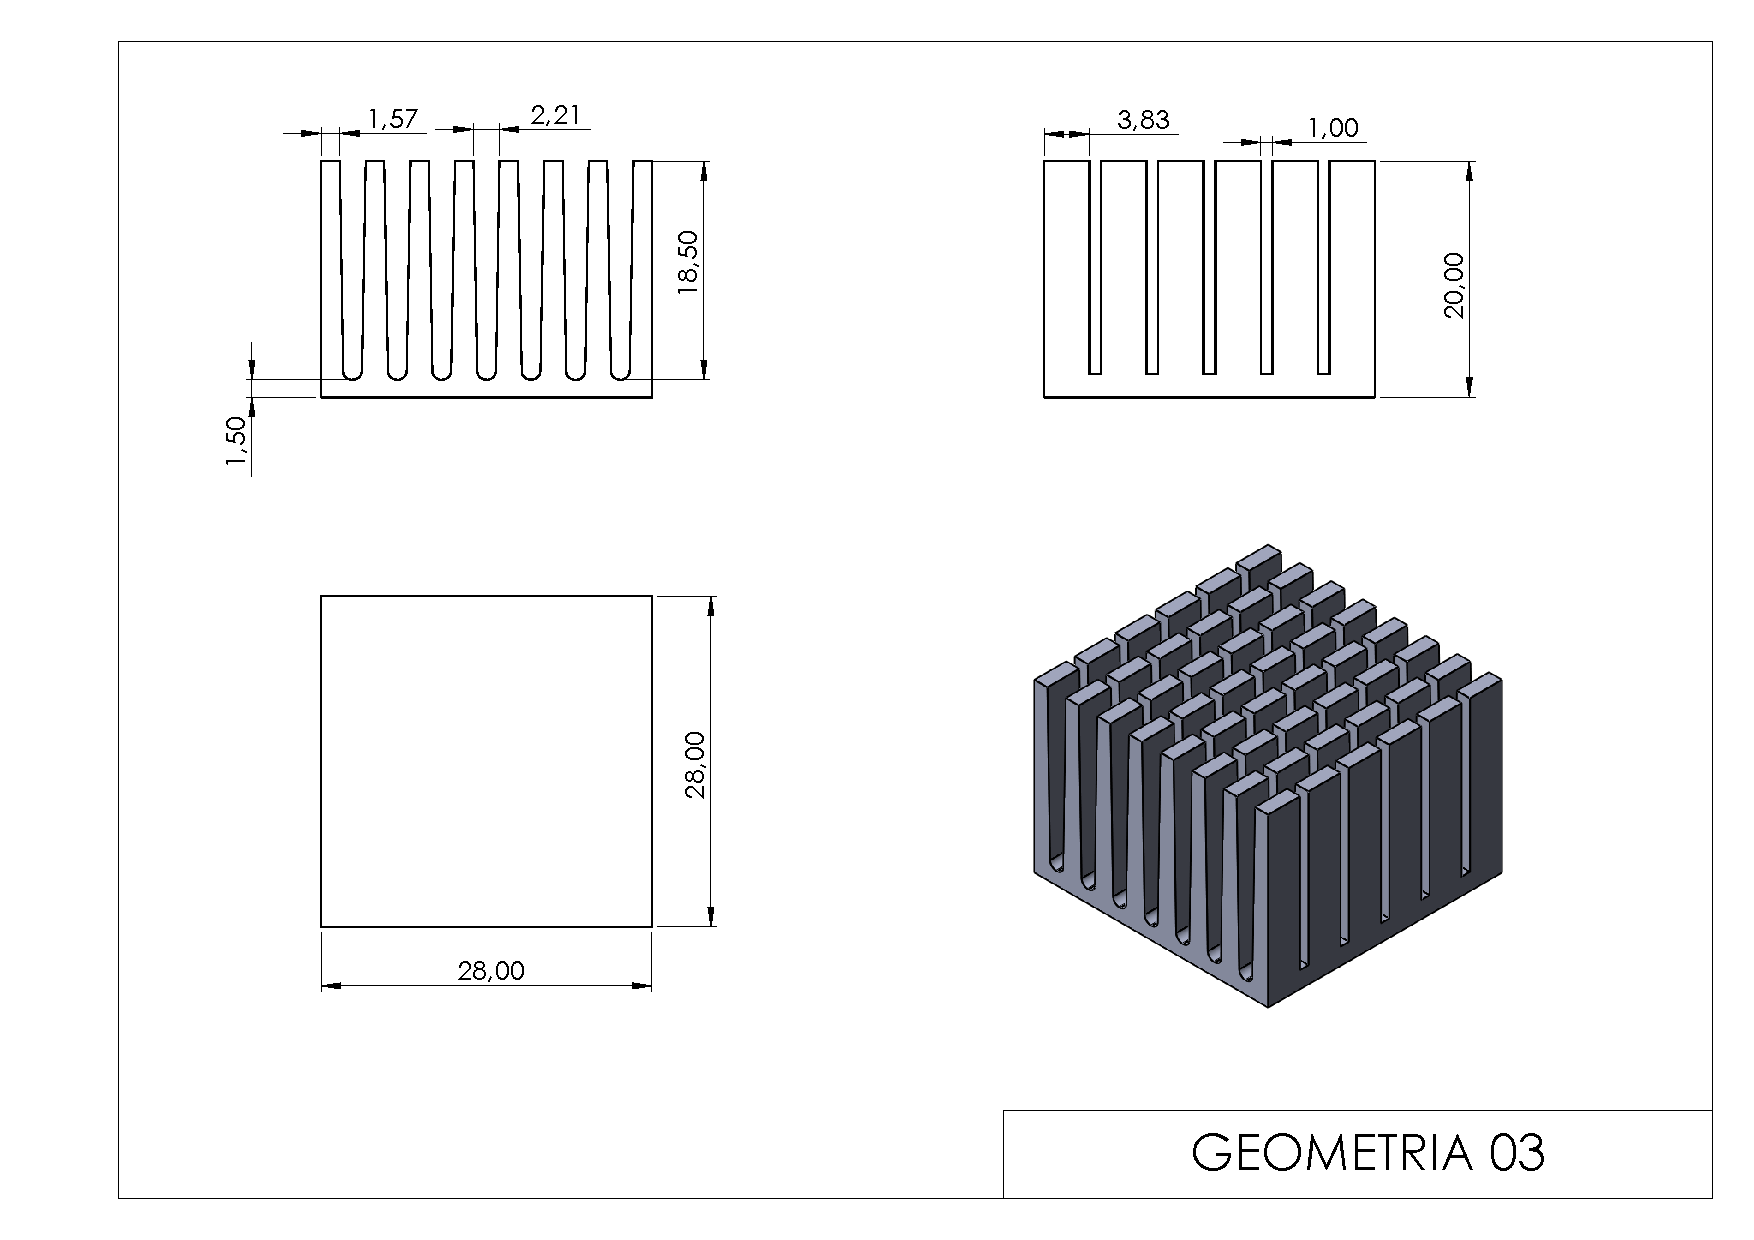
\includegraphics[width=15cm]{figuras/geometria.pdf}
    \fonteproprioautor
\end{figure}

Consideramos que a peça proposta será feita de alumínio, pelo fato do material ter um preço mais acessível e ter uma boa condução térmica, sendo amplamente utilizado na indústria para esse mesmo propósito.

\begin{figure}[h]
    \centering
    \caption{Tabela propriedades termofísicas de sólidos metálicos selecionados.}
    \label{fig:metalProps}
    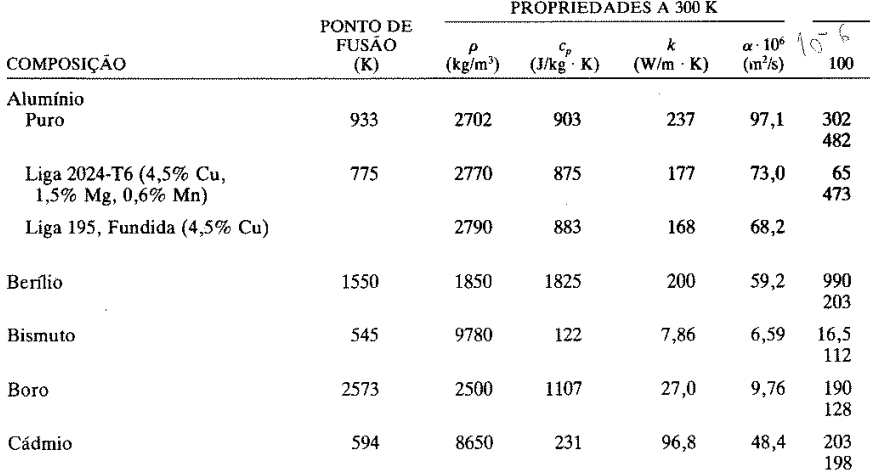
\includegraphics[width=14cm]{figuras/metalProps.jpg}
    \fonte{\citeonline{uspTabelasTermodinamicas}}
\end{figure}

Outras condições do funcionamento da condução térmica também foram pré-determinadas, sendo elas:

\begin{itemize}[leftmargin=2cm]
    \item Regime estacionário;
    \item Condutividade térmica constante;
    \item Radiação na superfície desprezível;
    \item Efeito de geração de calor ausentes;
    \item Coeficiente de transferência de calor h uniforme ao longo da superfície;
    \item Condições unidimensional na direção x;
    \item Transferência de calor por convecção.
\end{itemize}


\begin{table}[h]
    \ABNTEXfontereduzida
    \centering
    \caption{Grandezas fornecidas}
    \label{tab:grandezasFornecidas}
    \begin{tabular}{c c l}\toprule
        Grandeza    & Valor                                      & Descrição                                           \\
        \toprule
        k           & \SI{237}{\watt\per\meter\per\kelvin}       & Condutividade térmica do material - Alumínio        \\
        h           & \SI{20}{\watt\per\square\meter\per\kelvin} & Coeficiente de transferencia de calor por convecção \\
        T1          & \SI{110}\degreeCelsius                     & Temperatura da superficie                           \\
        T\(\infty\) & \SI{30}\degreeCelsius                      & Temperatura do ar ambiente                          \\
        Eb          & 0,0015 \SI{}{\meter}                       & Espessura da base                                   \\
        Lb          & 0,028 \SI{}{\meter}                        & Largura da base                                     \\
        Wb          & 0,028 \SI{}{\meter}                        & Profundidade da base                                \\
        ta          & 0,00157 \SI{}{\meter}                      & Espessura da aleta                                  \\
        La          & 0,0185 \SI{}{\meter}                       & Distância da base até na ponta da aleta             \\
        L total     & 0,02 \SI{}{\meter}                         & Altura total da peça                                \\
        Wa          & 0,00383 \SI{}{\meter}                      & Profundidade da aleta                               \\
        N           & 48un                                       & Quantidade de aletas                                \\
        e1          & 0,001 \SI{}{\meter}                        & Espaço entre as aletas pela frente                  \\
        e2          & 0,00221 \SI{}{\meter}                      & Espaço entre as aletas pelo lado                    \\
        \bottomrule
    \end{tabular}
    \fonteproprioautor
\end{table}
{\let\clearpage\relax\chapter{Cálculos}\label{cap:calculus}}
%\chapter{Cálculos}\label{cap:calculus}

\section{Cálculo para aleta Infinita}\label{sec:infity}

Realizado análise para aleta Infinita, obtida através da relação:\\
\begin{equation}
    {m}{L}\geq{2,65}
\end{equation}
\begin{equation}
    {L}\geq{\frac{2,65}{m}}
\end{equation}
\begin{equation}
    {L}\geq{\frac{2,65}{12,311 }}
\end{equation}
\begin{equation}
    {L}\geq{0,21522496\,\SI{}{\meter}}
\end{equation}
\par Para que hipótese da aleta infinita fosse válida, a aleta deveria ter um
comprimento maior ou igual a 21,522496 cm.
Neste caso a geometria 3 apresenta comprimento menor, embasando a
escolha da utilização do cálculo de contorno A.
\\
\\
{\ABNTEXchapterfont\Large{A) Determinar a temperatura da superfície da base da aleta (Tb)}}\\
%\section{Determinar a temperatura da superfície da base da aleta (Tb)}\label{sec:prob1}
Apropriando-se da equação da taxa de transferência de calor e isolando Tb (temperatura da base), com espessura da base em 0,0015m e taxa constante ao longo do eixo x, tem-se:
\begin{equation}
    {qx}={\frac{T\infty-Ts1}{1/{h1}}}={\frac{Ts1-Ts2}{L/{{k}{A}}}}={\frac{Ts2-T\infty2}{1/{h2}{A}}}
\end{equation}

\begin{figure}[h]
    \centering
    \caption{Representação das resistências térmicas.}
    \label{fig:res}
    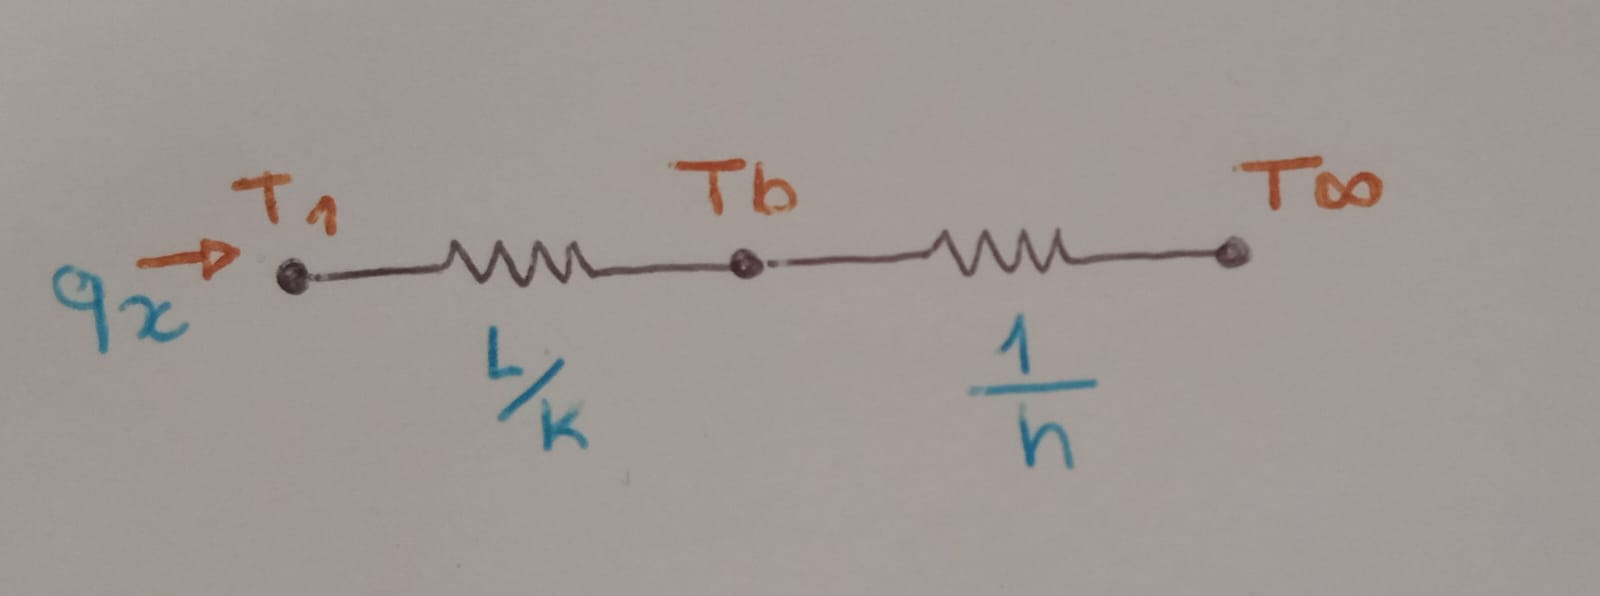
\includegraphics[width=10cm]{figuras/resistenciasTermicas.jpeg}
    \fonteproprioautor
\end{figure}

Isolando o Tb chegamos ao resultado de:
\begin{equation}
    {Tb}={\frac{T1 -T\infty}{{R1}+{R2}}}-{T1} = \SI{109,989}{\degreeCelsius}
\end{equation}
\\
{\ABNTEXchapterfont\Large{B) Determinar a taxa de transferência de calor de cada tipo de aleta (qa)}}
%\section{Determinar a taxa de transferência de calor de cada tipo de aleta (qa)}\label{sec:calcTable}

\begin{figure}[h]
    \centering
    \caption{Tabela com condições de cálculos para superfícies estendidas.}
    \label{fig:tabelaCasosCalc}
    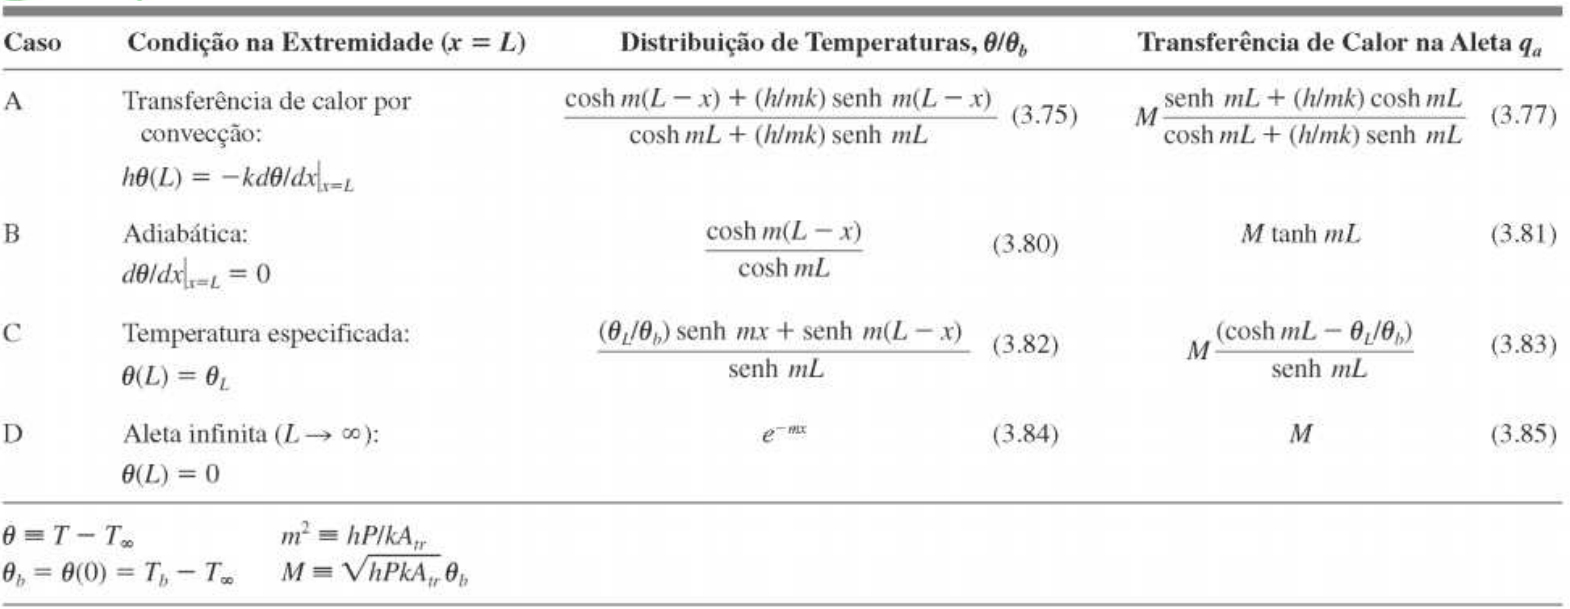
\includegraphics[width=15cm]{figuras/tabelaCasosCalc.jpg}
\end{figure}

Foi escolhida a equações do caso \(A\), pelo fato das equações
\(D\) aleta inifita resultar em um valor muito acima do comprimeto da
geometria,
\(B\) por não conter superfícies adiabáticas
e \(C\) por não conter uma temperatura especificada na parcela estendida.
\par No caso da equação \(A\), necessita-se dos seguintes valores
para prosseguimento com os cálculos:
\begin{itemize}[leftmargin=2cm]
    \item Perímetro da aleta: \(
          {P}={2w+2t} = \SI{10,8}{\milli\meter}
          \)
    \item Diferença de temperatura: \(
          {\theta}b={{Tb}-{T\infty}} = \SI{79,989}{\degreeCelsius}
          \)
    \item Área da seção transversal da aleta: \(
          {Atr}={{w}{t}} = \SI{12,311}{\per\meter}
          \)
    \item Valor \(M\): \(
          {M}={\sqrt[]{{h}{P}{k}{Atr}}} = \SI{1,403}{\watt}
          \)
    \item Taxa de transferência
          de calor da aleta: \\\(
          {qa}={M}{
          \frac
          {\sinh{(mLa)}+{\frac{(h)}{(mk)}}{\cosh{(mLa)}}}
          {\cosh{(mLa)}+{\frac{(h)}{(mk)}}{\sinh{(mLa)}}}
          }={0,3223\,\SI{}{\watt}}
          \)
\end{itemize}
{\ABNTEXchapterfont\Large\vspace{1cm}{C) Determinar a temperatura na ponta da aleta}}
%\section{Determinar a temperatura na ponta da aleta}\label{sec:C}
\begin{equation}
    {\frac{\theta}{{\theta}b}}=
    {\frac
    {T(x)-{T\infty}}
    {Tb-{T\infty}}
    }=
    {
    \frac
    {\cosh{(m(L-x))}+{\frac{(h)}{(mk)}}{\sinh{(m(L-x))}}}
    {\cosh{(mL)}+{\frac{(h)}{(mk)}}{\sinh{(m(L-x))}}}
    }
\end{equation}
Isolando o \(tx\) obtém-se:
\begin{equation}
    {Ta(x)}=
    {
    \frac
    {\cosh{(m(L-x))}+{\frac{(h)}{(mk)}}{\sinh{(m(L-x))}}}
    {\cosh{(mL)}+{\frac{(h)}{(mk)}}{\sinh{(m(L-x))}}}
    }+
    {\theta}+
    {T\infty}=
    \SI{107,839}{\degreeCelsius}
\end{equation}
\\
{\ABNTEXchapterfont\Large{D) Determinar a efetividade (\(\epsilon\)) da superfície estendida}}\\
%\section{ Determinar a efetividade (\(\epsilon\)) da superfície estendida}\label{sec:d}
É a razão entre a taxa de transferência de calor da aleta e a taxa de
transferência de calor que existiria sem a presença da aleta
\begin{equation}
    {{\epsilon}a}=
        {
            \frac
            {{qa1}}
            {{h}{Atrb}{\theta}b}
        }=
        {\SI{33,613}{}}
\end{equation}
\par Não houve a necessidade de realizar melhorias, pois \({\epsilon}a>{2}\).
\\
\\
{\ABNTEXchapterfont\Large{E) Determinar a eficiência da aleta (\(\eta\)a)}}
%\section{Determinar a eficiência da aleta (\(\eta\)a)}\label{sec:e}

\begin{itemize}[leftmargin=2cm]
    \item Áreas das aletas: \(
          {Aa}={{L1}{P}+{Atr}} = 0,0002058131\,\SI{}{\square\meter}
          \)
    \item Eficiência da aleta: \(
          {\eta}a=
          {\frac{qa}{{h}{Aa}{\theta}b}}{100\%}=
          {\SI{98,20}{\percent}}
          \)
\end{itemize}.
\\
\\
{\ABNTEXchapterfont\Large{F) Determinar a eficiência global do conjunto aletado (\(\eta\)o)}}
%\section{Determinar a eficiência global do conjunto aletado (\(\eta\)o)}\label{sec:f}

\par O conjunto aletado global compreende toda a geometria desde a base até todas as superfícies estendidas e 
para determinarmos a eficiência de todo esse conjunto
apenas necessita-se somar a energia transmitida da base
como a energia dissipada por todas as aletas.
A eficiência provem da razão entre da energia  dissipada e a energia transportada por convecção:

\begin{itemize}[leftmargin=2cm]
    \item Área total (aletas + espaço sem aletas): \(
          {At}={{Aa}{N}+{Ab}} = {0,0112849}\,\SI{}{\square\meter}
          \)
    \item Taxa total da transferência de calor: \(
          {qt}=
          {{N}{{\eta}a}{h}{Aa}{{\theta}b}}+{{h}{Ab}{{\theta}b}}=
              {17,769\,\SI{}\watt}
          \)
    \item Eficiência global do conjunto aletado: \(
          {\eta}o=
          {\frac{qt}{{h}{At}{\theta}b}}{100\%}=
          {\SI{98,43}{\percent}}
          \)
\end{itemize}

\section{
  Resultados
 }\label{sec:results}

O resultados foram satisfatórios pois a aleta apresentou valores de:
\begin{itemize}[leftmargin=2cm]
    \item Efetividade \boldmath\(> 2\), não havendo a necessidade realizar melhorias;
    \item Eficiência global de \boldmath\(98,43\,\%\).
\end{itemize}
\chapter{Conclusões}\label{cap:conclusoes}

Este trabalho procurou mostrar como deverá ser a apresentação da monografia a ser submetida à Coordenação do Curso de Engenharia de Telecomunicações do \gls{IFSC} para a obtenção do diploma de Bacharel em Engenharia de Telecomunicações.

No \autoref{cap:introducao} foi feita uma pequena introdução. No \autoref{cap:revisao} foi apresentado o uso de alguns ambientes flutuantes no~\LaTeX~. E no \autoref{cap:proposta} foi apresentado sobre equações e como inserir trechos de código.

Como trabalho futuro, fica a reescrita do texto deste documento de forma que ele possam indicar informações específicas a formatação do documento. Como o tamanho da fonte utilizada, o espaçamento da borda, o alinhamento e numeração das seções e capítulos etc.



%-----------------------------------------------%
% ELEMENTOS PÓS-TEXTUAIS
%-----------------------------------------------%
\postextual
% %-----------------------------------------------%
%-----------------------------------------------%
% Referências bibliográficas
%-----------------------------------------------%
\bibliography{referencias}


%-----------------------------------------------%
% Apêndices
%-----------------------------------------------%
\begin{apendicesenv}
% Imprime uma página indicando o início dos apêndices
\partapendices

\chapter{Meu primeiro apêndice}

Texto ou documento, elaborado pelo autor, a fim de complementar sua argumentação, sem prejuízo da unidade nuclear do trabalho. Os apêndices são identificados por letras maiúsculas ordenadas alfabeticamente, travessão e pelo respectivo título. 

\end{apendicesenv}

%-----------------------------------------------%
% Anexos
%-----------------------------------------------%
\begin{anexosenv}
% Imprime uma página indicando o início dos anexos
\partanexos

\chapter{Meu primeiro assunto de anexo}

Texto ou documento não elaborado pelo autor, que serve de fundamentação, comprovação e ilustração. Os anexos são identificados por letras maiúsculas ordenadas alfabeticamente, travessões e pelos respectivos títulos. 


\chapter{Segundo assunto que pesquisei}
\lipsum[31]

\end{anexosenv}


    
\end{document}

